%!TEX program = xelatex 
%!TEX encoding = UTF-8 unicode
\documentclass[UTF8,nofonts]{ctexart}
\setCJKmainfont[BoldFont=STHeiti,ItalicFont=STKaiti]{STSong}
\setCJKsansfont[BoldFont=STHeiti]{STXihei}
\setCJKmonofont{STFangsong}
\setcounter{secnumdepth}{5}
\usepackage[hmarginratio=1:1]{geometry}
\usepackage{array,float,graphicx}
\usepackage{pstricks-add}
% \usepackage{minted}
\usepackage{hyperref}
\usepackage{color,subfigure}
\usepackage{amsmath}
\usepackage{ulem,diagbox}
%表格style
\newcolumntype{L}[1]{>{\vspace{0.5em}\begin{minipage}{#1}\raggedright\let\newline\\
\arraybackslash\hspace{0pt}}m{#1}<{\end{minipage}\vspace{0.5em}}}
\newcolumntype{R}[1]{>{\vspace{0.5em}\begin{minipage}{#1}\raggedleft\let\newline\\
\arraybackslash\hspace{0pt}}m{#1}<{\end{minipage}\vspace{0.5em}}}
\newcolumntype{C}[1]{>{\vspace{0.5em}\begin{minipage}{#1}\centering\let\newline\\
\arraybackslash\hspace{0pt}}m{#1}<{\end{minipage}\vspace{0.5em}}}
%
\makeatletter
\renewcommand{\section}{
\@startsection{section}{1}{0mm}{-\baselineskip}{0.5\baselineskip}{\fontsize{16pt}{16pt}\bf\leftline}
}
\newcommand{\bhref}[2]{
\textcolor{blue}{\href{#1}{#2}}
}
\newcommand*\xor{\mathbin{\oplus}}
\newcommand*\mylshift{<\kern -.3em <}
\definecolor{bg}{rgb}{0.95,0.95,0.95}
\makeatother
%引用style
\makeatletter
\def\@cite#1#2{\textsuperscript{[{#1\if@tempswa , #2\fi}]}}
\makeatother
\pagestyle{empty}
%封面
\title{
\fontsize{26pt}{26pt}
天气应用需求报告与设计报告
%垂直间距
\vskip 20em
}
\author{
软件工程1102班 \ \ \ 靳杰 \ \ \ U201112375
}
\date{}
\thispagestyle{empty}

\begin{document}
\maketitle
\thispagestyle{empty}
\newpage
\section{天气应用需求分析}
\subsection{需求描述}
基于iOS手机操作系统,制作一款天气应用,实现以下基本功能点:

\begin{itemize}
 	\item 从中国天气网,webservice获取指定的城市天气信息,并可在系统中显示当前天气情况。
 	\item 用sqlite数据库保存获取的历史天气信息,查阅存储的历史天气。
 	\item 对以往的天气情况进行统计,各类天气的数量,百分比。
 	\item 绘制温度的变化曲线图。
\end{itemize} 

\subsection{需求分析}
\subsubsection{应用范围} % (fold)
\label{ssub:应用范围}
系统运行在iOS移动操作系统平台上,要求iOS 7.0及以上。适用机型:iPhone4、iPhone4s、iPhone5、iPhone5s。
% subsubsection 应用范围_ (end)
\subsubsection{应用功能点定义} % (fold)
\label{ssub:应用功能定义_}
\begin{itemize}
	\item 定位当前城市,显示当前天气情况。
	\item 更改城市,显示指定城市天气情况。
	\item 绘制温度变化曲线图。
	\item 查询存储的天气情况。
\end{itemize}
% subsubsection 应用功能定义_ (end)
% subsection 需求分析_ (end)

\section{系统设计} % (fold)
\label{sec:系统设计_}

% section 系统设计_ (end)

\section{系统截图展示} % (fold)
\label{sec:系统截图展示_}
\begin{figure}[hbt]
\centering

\includegraphics[width=0.8\textwidth]{1.png}
\caption{系统欢迎界面}
\end{figure}
\begin{figure}[hbt]
\centering

\includegraphics[width=0.8\textwidth]{2.png}
\caption{系统启动界面}
\end{figure}
\begin{figure}[hbt]
\centering
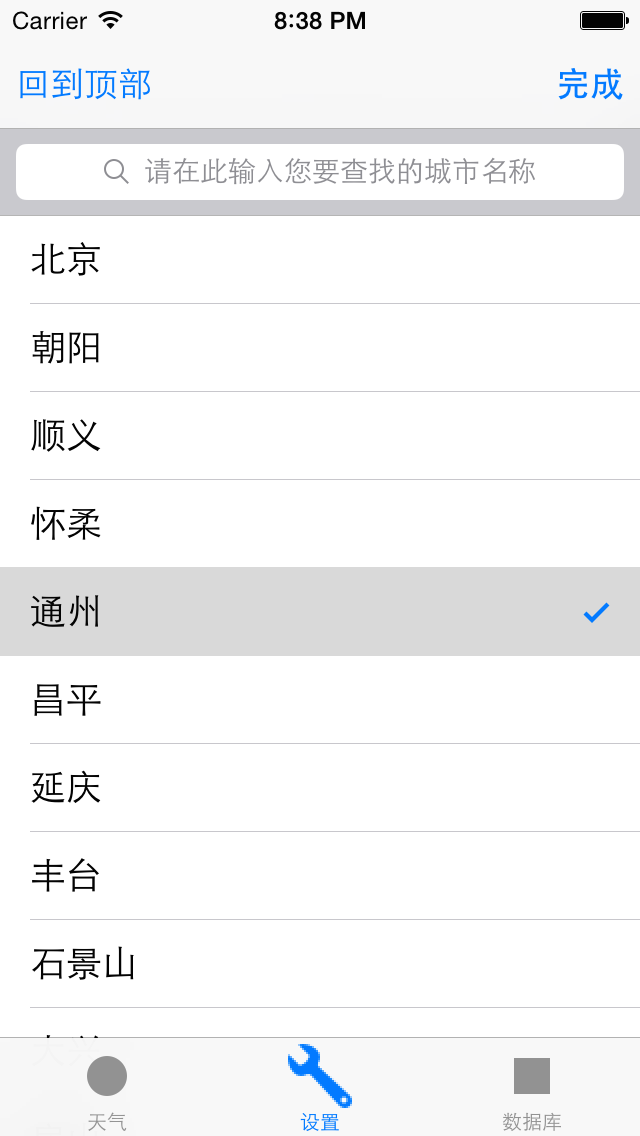
\includegraphics[width=0.8\textwidth]{3.png}
\caption{城市选择界面}
\end{figure}
\begin{figure}[hbt]
\centering
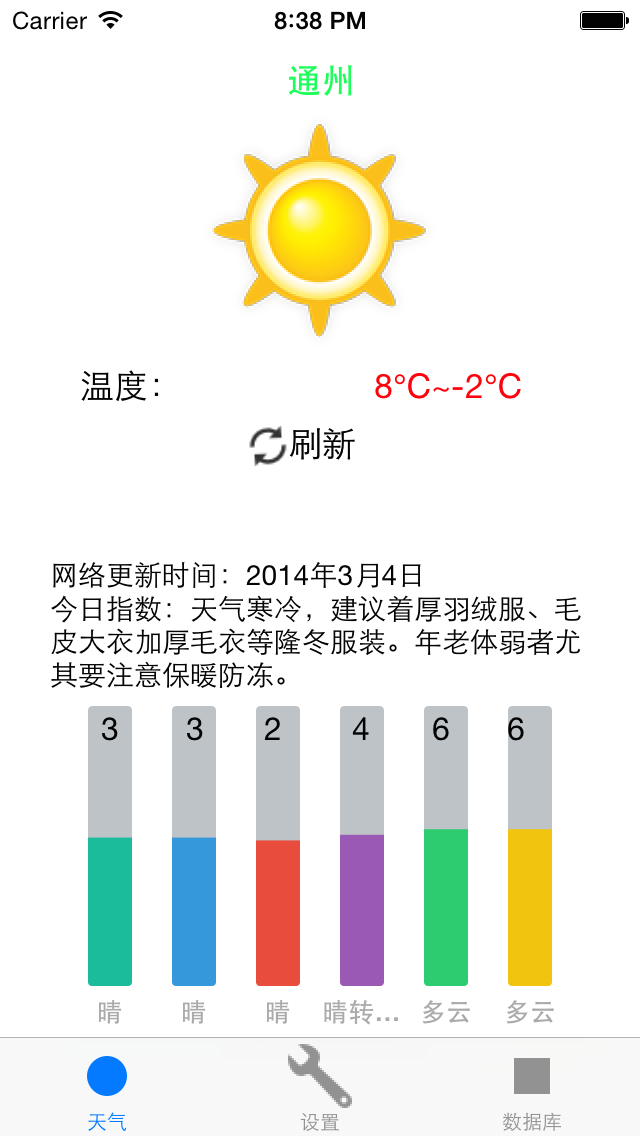
\includegraphics[width=0.8\textwidth]{4.png}
\caption{选择城市后更新界面}
\end{figure}
\begin{figure}[hbt]
\centering
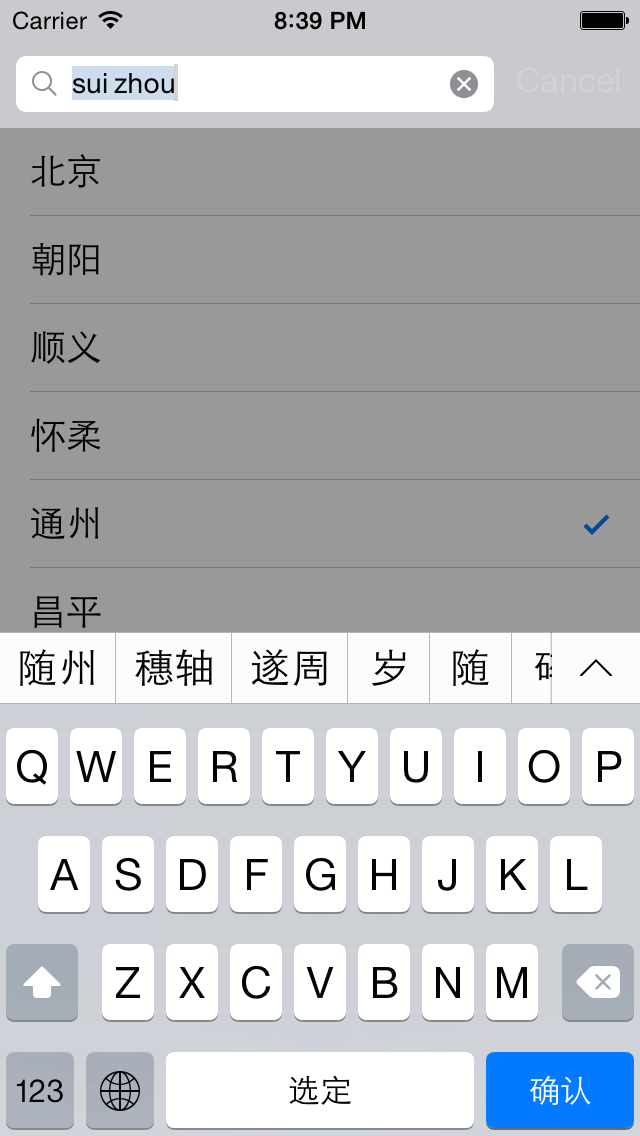
\includegraphics[width=0.8\textwidth]{5.png}
\caption{城市搜索界面}
\end{figure}
\begin{figure}[hbt]
\centering
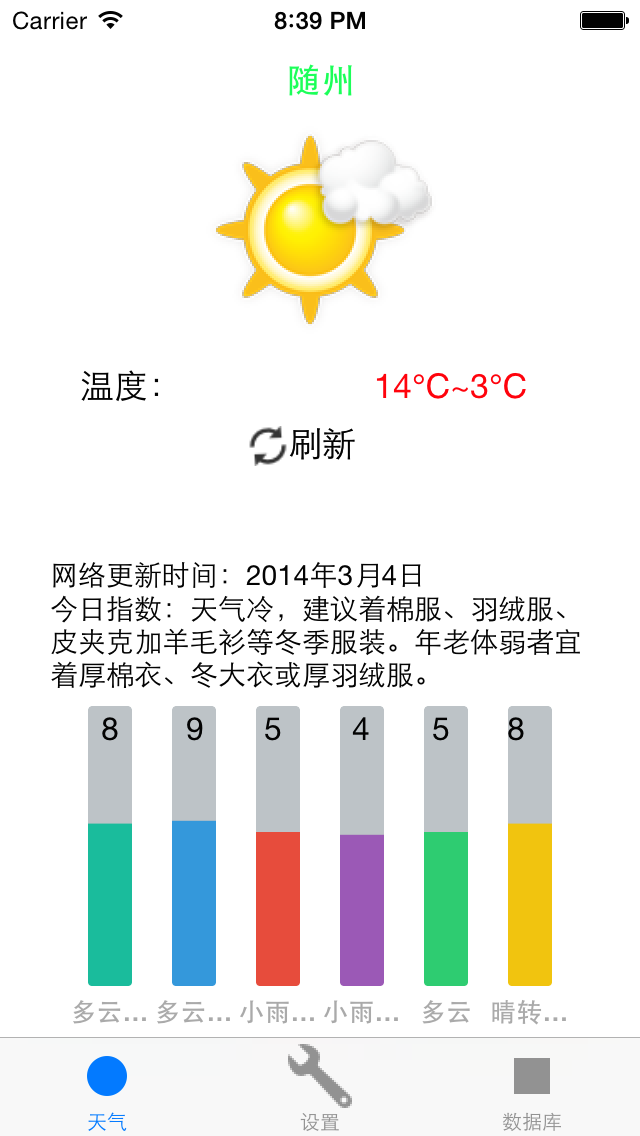
\includegraphics[width=0.8\textwidth]{6.png}
\caption{搜索后更新界面}
\end{figure}
\begin{figure}[hbt]
\centering
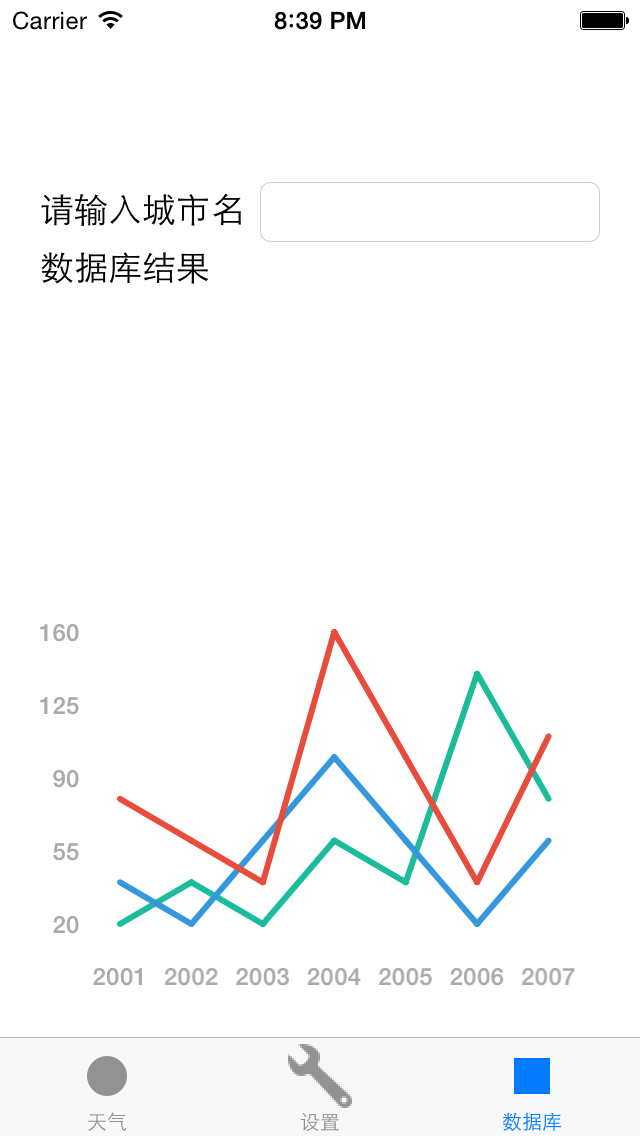
\includegraphics[width=0.8\textwidth]{7.png}
\caption{数据库界面}
\end{figure}
\begin{figure}[hbt]
\centering

\includegraphics[width=0.8\textwidth]{8.png}
\caption{系统搜索界面}
\end{figure}
\begin{figure}[hbt]
\centering

\includegraphics[width=0.8\textwidth]{9.png}
\caption{系统搜索结果界面}
\end{figure}
% section 系统截图展示_ (end)
\end{document}